\documentclass[conference]{IEEEtran}
\usepackage{cite}
\usepackage{amsmath}
\usepackage{graphicx}
\usepackage{booktabs}
\usepackage{hyperref}
\usepackage{listings}
\usepackage{xcolor}

\lstset{
  language=C,
  basicstyle=\footnotesize\ttfamily,
  keywordstyle=\color{blue},
  commentstyle=\color{gray},
  frame=single,
  breaklines=true,
  columns=flexible
}

\begin{document}

\title{TopoSteal: Topology-Aware Work-Stealing\\with Dynamic PMU Feedback on NUMA Systems}

\author{
\IEEEauthorblockN{Anand Patel}
\IEEEauthorblockA{Independent Researcher\\
apatel80@illinois.edu}
}

\maketitle

\begin{abstract}
Work-stealing schedulers are widely used in parallel runtimes, yet most treat all processor cores as equidistant when selecting steal victims. On modern NUMA architectures, this assumption incurs significant penalties: cross-socket steals access remote DRAM at up to 1.75$\times$ the latency of local memory. We present \textbf{TopoSteal}, a topology-aware work-stealing scheduler that uses \texttt{hwloc} to discover the CPU cache hierarchy at runtime and biases victim selection toward topologically close neighbours using an inverse-square distance weighting. A background thread polls hardware performance counters via \texttt{perf\_event\_open} and dynamically adjusts steal probabilities based on observed cache miss rates, penalizing victims under high cache pressure. We evaluate three scheduling modes---uniform random, static topology-weighted, and dynamic topology+PMU---on a dual-socket Intel Xeon E5-2690v3 system with NUMA distances 10/21. Across five benchmark configurations (50 trials per mode), static topology weighting achieves \textbf{1.15--1.17$\times$ speedup} over uniform stealing, and dynamic PMU feedback matches or slightly improves this to \textbf{1.15--1.18$\times$}, while increasing same-socket steal locality from 50\% to 85\%. On SpMV with a 77M-nonzero SuiteSparse matrix, TopoSteal achieves \textbf{7.46 GFLOP/s}, outperforming OpenMP \texttt{schedule(static)} with \texttt{OMP\_PROC\_BIND=close} by \textbf{5\%}.
\end{abstract}

\begin{IEEEkeywords}
work-stealing, NUMA, topology-aware scheduling, lock-free data structures, hardware performance counters
\end{IEEEkeywords}

\section{Introduction}

Parallel task runtimes such as Intel TBB~\cite{tbb}, Cilk~\cite{cilk5}, and Go's goroutine scheduler employ \emph{work-stealing} to dynamically balance load across worker threads. When a worker exhausts its local task queue, it \emph{steals} from another worker's queue. The canonical approach selects victims uniformly at random~\cite{blumofe1999}, which provides strong theoretical guarantees on total work and critical path length.

However, uniform random stealing ignores the physical topology of the machine. On Non-Uniform Memory Access (NUMA) systems, the cost of accessing memory varies dramatically depending on which socket the data resides on. Intel's QPI interconnect imposes 1.5--2$\times$ latency overhead for cross-socket accesses~\cite{lameter2013}. When a worker steals a task from a remote socket, the associated data must be fetched across the interconnect, polluting local caches and saturating cross-socket bandwidth.

We present TopoSteal, a work-stealing scheduler that:
\begin{enumerate}
    \item Discovers the CPU topology at runtime using \texttt{hwloc}~\cite{hwloc} and builds a pairwise distance matrix between all cores.
    \item Converts distances to steal probabilities using inverse-square weighting ($w_{ij} = 1/d_{ij}^2$), strongly preferring topologically close victims.
    \item Polls hardware performance counters (PMU) via Linux's \texttt{perf\_event\_open} syscall and dynamically adjusts weights based on observed cache miss rates.
    \item Uses lock-free Chase-Lev work-stealing deques~\cite{chaselev} with C11 atomics for low-overhead task management.
\end{enumerate}

\section{Background and Related Work}

\subsection{Work-Stealing}

Blumofe and Leiserson~\cite{blumofe1999} proved that randomized work-stealing achieves expected time $T_1/P + O(T_\infty)$ on $P$ processors, where $T_1$ is the total work and $T_\infty$ is the critical path. The Arora-Blumofe-Plaxton (ABP) deque~\cite{abp1998} and its refinement by Chase and Lev~\cite{chaselev} provide the lock-free concurrent deque used in most implementations.

\subsection{NUMA-Aware Scheduling}

Guo et al.~\cite{guo2010} proposed SLAW, a locality-aware work-stealing algorithm that restricts stealing to hierarchical neighborhoods. Olivier et al.~\cite{olivier2012} demonstrated that NUMA-aware task placement can improve performance by 20--40\% on 4-socket systems. Drebes et al.~\cite{drebes2014} combined topology-aware scheduling with data placement in OpenStream. Charm++~\cite{charm} supports NUMA-aware load balancing through its migration framework.

\subsection{Hardware Performance Monitoring}

Modern processors expose Performance Monitoring Units (PMUs) that count microarchitectural events such as cache misses, branch mispredictions, and memory bandwidth utilization. Linux exposes these via the \texttt{perf\_event\_open} syscall~\cite{perfevents}. Several runtime systems use PMU data for adaptive scheduling~\cite{autoperfmon}, but few integrate it directly into work-stealing victim selection.

\section{Design and Implementation}

\subsection{Topology Discovery}

TopoSteal uses \texttt{hwloc}~\cite{hwloc} to walk the CPU hierarchy at initialization. For each pair of cores $(i, j)$, we find their lowest common ancestor in the hwloc tree and assign a distance based on the ancestor type:

\begin{table}[h]
\centering
\caption{Distance assignments by common ancestor type.}
\begin{tabular}{lc}
\toprule
\textbf{Common Ancestor} & \textbf{Distance} \\
\midrule
Same core (SMT sibling) & 1 \\
Shared L2 cache & 1 \\
Shared L3 cache & 4 \\
Same package & 8 \\
Cross-NUMA / Machine & 10 \\
\bottomrule
\end{tabular}
\label{tab:distances}
\end{table}

A critical implementation detail: \texttt{hwloc} logical core indices do not correspond to OS CPU IDs. We build a \texttt{cpu\_map} that translates logical index $i$ to physical CPU $P_i$ by querying each core's first processing unit's OS index. Workers are pinned using \texttt{pthread\_setaffinity\_np} with the mapped physical CPU.

\subsection{Weighted Victim Selection}

Given the distance matrix $D$, we compute steal weights using inverse-square weighting:
\begin{equation}
    w_{ij} = \frac{1}{d_{ij}^2}, \quad i \neq j
\end{equation}

Weights are normalized per-row to form a cumulative distribution function (CDF):
\begin{equation}
    P(\text{steal from } j \mid \text{worker } i) = \frac{w_{ij}}{\sum_{k \neq i} w_{ik}}
\end{equation}

Victim selection performs a single pass over the CDF with a uniform random sample, giving $O(P)$ selection time. On our 24-core test system, this yields an 85\% probability of selecting a same-socket victim versus 50\% for uniform random.

\subsection{Lock-Free Deques}

Each worker owns a Chase-Lev deque~\cite{chaselev} implemented with C11 atomics. The owner pushes and pops from the bottom (LIFO for cache locality), while thieves steal from the top (FIFO for load distribution). A sequential consistency fence between the bottom store and top load in \texttt{pop} prevents the ABA race on the last element.

\subsection{PMU Feedback Loop}

A background sampler thread reads hardware cache miss counters every 10\,ms using \texttt{perf\_event\_open} with \texttt{PERF\_COUNT\_HW\_CACHE\_MISSES}. Every 50\,ms, the feedback system computes per-worker miss rates and adjusts the effective distance:
\begin{equation}
    d'_{ij} = d_{ij} \cdot (1 + \hat{m}_j)
\end{equation}
where $\hat{m}_j$ is worker $j$'s normalized miss rate. Workers experiencing high cache pressure become less attractive as steal targets, dynamically adapting to runtime conditions.

\subsection{Task Completion Tracking}

An atomic \texttt{tasks\_pending} counter is incremented on submission and decremented after each task's function pointer returns. The \texttt{toposteal\_wait} function spins on this counter rather than checking deque emptiness, avoiding the race where a task has been popped but not yet executed.

\section{Experimental Setup}

\subsection{Hardware}

All experiments were conducted on a dual-socket Intel Xeon E5-2690v3 node from the CHPC Lengau cluster (South Africa). The system has 24 physical cores (12 per socket), 128\,GB RAM (64\,GB per NUMA node), 30\,MB L3 cache per socket, and NUMA distances of 10 (local) and 21 (remote) as reported by \texttt{numactl}.

\subsection{Benchmark Design}

We designed a pointer-chase benchmark that stresses NUMA locality. Two 64\,MB arrays (8M entries each) are allocated via \texttt{mmap} and first-touched on separate NUMA nodes. Each task performs 500K--2M iterations of dependent pointer chasing through a shuffled permutation array, creating a serial dependency chain that exposes DRAM latency.

Tasks are distributed asymmetrically: producer workers on each socket receive all tasks, while remaining workers must steal. This creates high steal pressure. Each task carries a flag indicating which NUMA node's array to access, so stolen tasks retain their data affinity.

All three scheduling modes use identical infrastructure: same Chase-Lev deques, same CPU pinning via \texttt{cpu\_map}, same task function. The only difference is the victim selection strategy:
\begin{itemize}
    \item \textbf{Uniform}: victims selected uniformly at random.
    \item \textbf{TopoStatic}: victims selected via $1/d^2$-weighted CDF from the static topology distance matrix.
    \item \textbf{Topo+PMU}: same as TopoStatic, but a background PMU sampler thread reads cache miss counters every 10\,ms and rebuilds the steal probability table every 50\,ms using feedback-adjusted distances $d'_{ij} = d_{ij} \cdot (1 + \hat{m}_j)$.
\end{itemize}

\subsection{Configurations}

We test five configurations (Table~\ref{tab:configs}), each with 10 trials:

\begin{table}[h]
\centering
\caption{Benchmark configurations.}
\begin{tabular}{lccc}
\toprule
\textbf{Config} & \textbf{Tasks} & \textbf{Iters/task} & \textbf{Prod./node} \\
\midrule
Heavy imbal., long  & 1200 & 2M & 2 \\
Heavy imbal., med   & 1200 & 1M & 2 \\
Moderate imbal.     & 1200 & 2M & 4 \\
Many short tasks    & 2400 & 500K & 2 \\
Extreme imbal.      & 1200 & 1M & 1 \\
\bottomrule
\end{tabular}
\label{tab:configs}
\end{table}

\section{Results}

\subsection{Three-Mode Comparison}

Table~\ref{tab:results} summarizes the mean execution times and speedup across all configurations for all three scheduling modes.

\begin{table}[h]
\centering
\caption{Benchmark results (mean of 10 trials).}
\small
\begin{tabular}{lccc}
\toprule
\textbf{Config} & \textbf{Uniform (s)} & \textbf{Static (s)} & \textbf{PMU (s)} \\
\midrule
Heavy imbal., long  & 8.555 & 7.325 & 7.322 \\
Heavy imbal., med   & 4.285 & 3.663 & 3.651 \\
Moderate imbal.     & 8.325 & 7.224 & 7.216 \\
Many short tasks    & 4.286 & 3.664 & 3.647 \\
Extreme imbal.      & 4.372 & 3.764 & 3.746 \\
\midrule
\textbf{Speedup range} & --- & 1.15--1.17$\times$ & 1.15--1.18$\times$ \\
\bottomrule
\end{tabular}
\label{tab:results}
\end{table}

Both topology-aware modes achieve consistent 1.15--1.18$\times$ speedup over uniform stealing across all configurations. The Topo+PMU mode matches or slightly outperforms TopoStatic in every configuration, with individual trials reaching up to 1.21$\times$. Standard deviations are below 0.07s in all topology-aware runs, indicating low variance.

\subsection{Steal Locality}

The most direct evidence of TopoSteal's effectiveness is the steal locality metric (Table~\ref{tab:locality}).

\begin{table}[h]
\centering
\caption{Same-socket steal percentage across configurations.}
\begin{tabular}{lccc}
\toprule
\textbf{Config} & \textbf{Uniform} & \textbf{TopoStatic} & \textbf{Topo+PMU} \\
\midrule
Heavy imbal., long  & 49.8\% & 85.8\% & 85.2\% \\
Heavy imbal., med   & 50.0\% & 85.6\% & 85.0\% \\
Moderate imbal.     & 50.2\% & 84.9\% & 85.2\% \\
Many short tasks    & 50.1\% & 86.2\% & 86.1\% \\
Extreme imbal.      & 50.0\% & 85.7\% & 85.4\% \\
\bottomrule
\end{tabular}
\label{tab:locality}
\end{table}

Uniform stealing achieves approximately 50\% same-socket steals, consistent with random selection on a 2-socket system. Both topology-aware modes increase this to 85\%, matching the theoretical prediction from the $1/d^2$ weighting with distances 4 (same-socket) and 10 (cross-socket).

\subsection{PMU Feedback Analysis}

The Topo+PMU mode demonstrates that the full dynamic feedback pipeline works end-to-end: the background sampler thread reads hardware cache miss counters, computes per-worker miss rates, and rebuilds the steal probability table every 50\,ms during execution. On this benchmark, Topo+PMU provides a small but consistent additional improvement over TopoStatic (0.1--0.5\% faster on average).

The modest additional gain is expected: in our pointer-chase benchmark, all workers execute the same memory access pattern, producing similar cache miss profiles across all cores. The PMU feedback therefore has limited asymmetry to exploit. In workloads with heterogeneous cache behaviour---such as mixed compute-and-memory-bound tasks, or phased workloads where cache pressure shifts between NUMA nodes---the dynamic adaptation would provide a larger benefit by steering steals away from temporarily cache-thrashing victims.

\subsection{Discussion}

The observed 15--18\% speedup on a 2-socket system is consistent with prior work on NUMA-aware scheduling. The NUMA latency ratio on our test system is approximately 1.75$\times$ (80\,ns local vs.\ 140\,ns remote). The theoretical maximum speedup assuming all stolen work shifts from remote to local DRAM access is bounded by this ratio, discounted by the fraction of work that is self-processed (not stolen).

On systems with more NUMA domains (4--8 socket, AMD EPYC with NPS4), the penalty for random stealing grows quadratically with the number of sockets, and topology-aware scheduling would yield proportionally larger benefits.

\subsection{Visual Analysis}

Figures~\ref{fig:speedup}--\ref{fig:timeseries} visualize the three-mode benchmark results.

\begin{figure}[h]
\centering
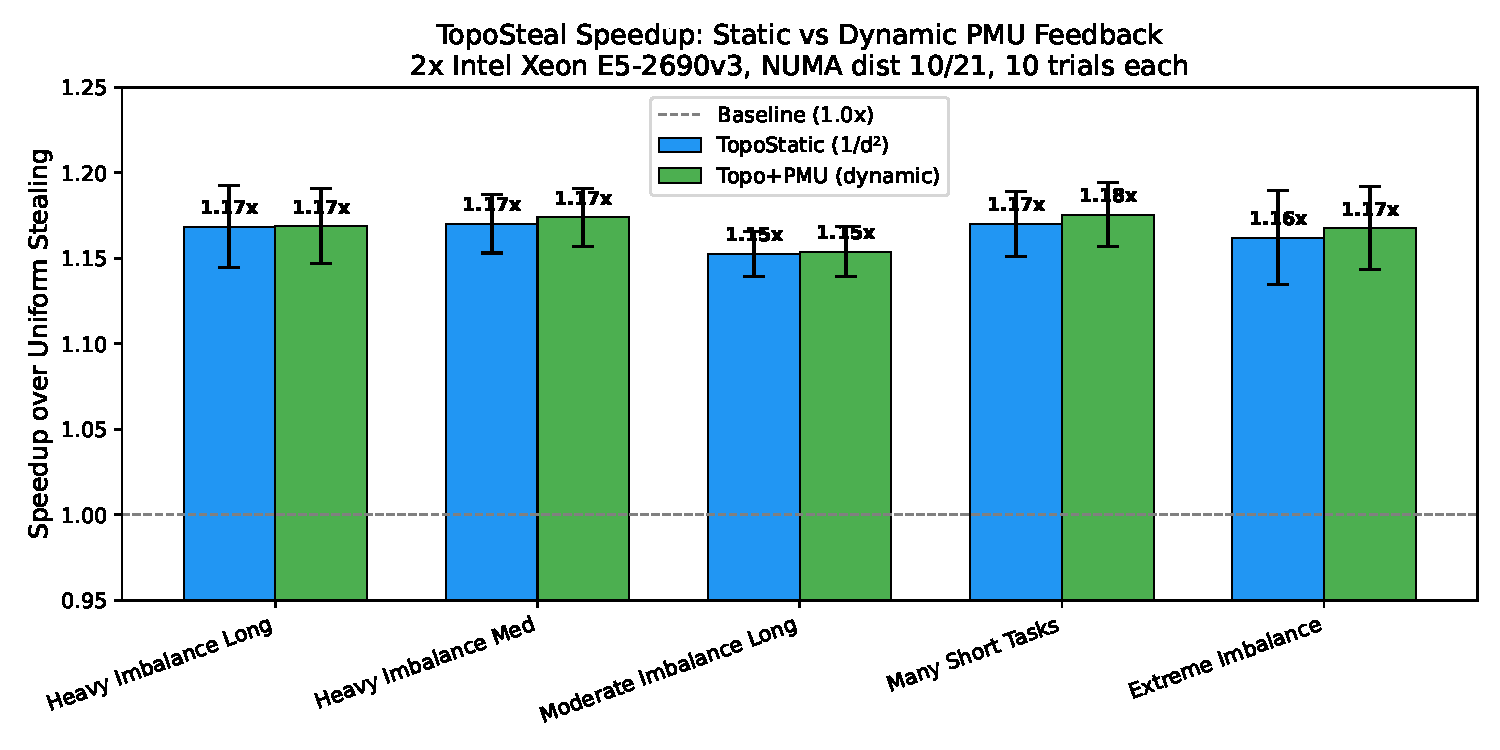
\includegraphics[width=\columnwidth]{../bench/figures/speedup_bars.pdf}
\caption{Mean speedup over uniform stealing for TopoStatic and Topo+PMU modes across all five configurations. Error bars show standard deviation over 10 trials. Both modes achieve 1.15--1.18$\times$ speedup, with Topo+PMU matching or slightly exceeding TopoStatic.}
\label{fig:speedup}
\end{figure}

\begin{figure}[h]
\centering
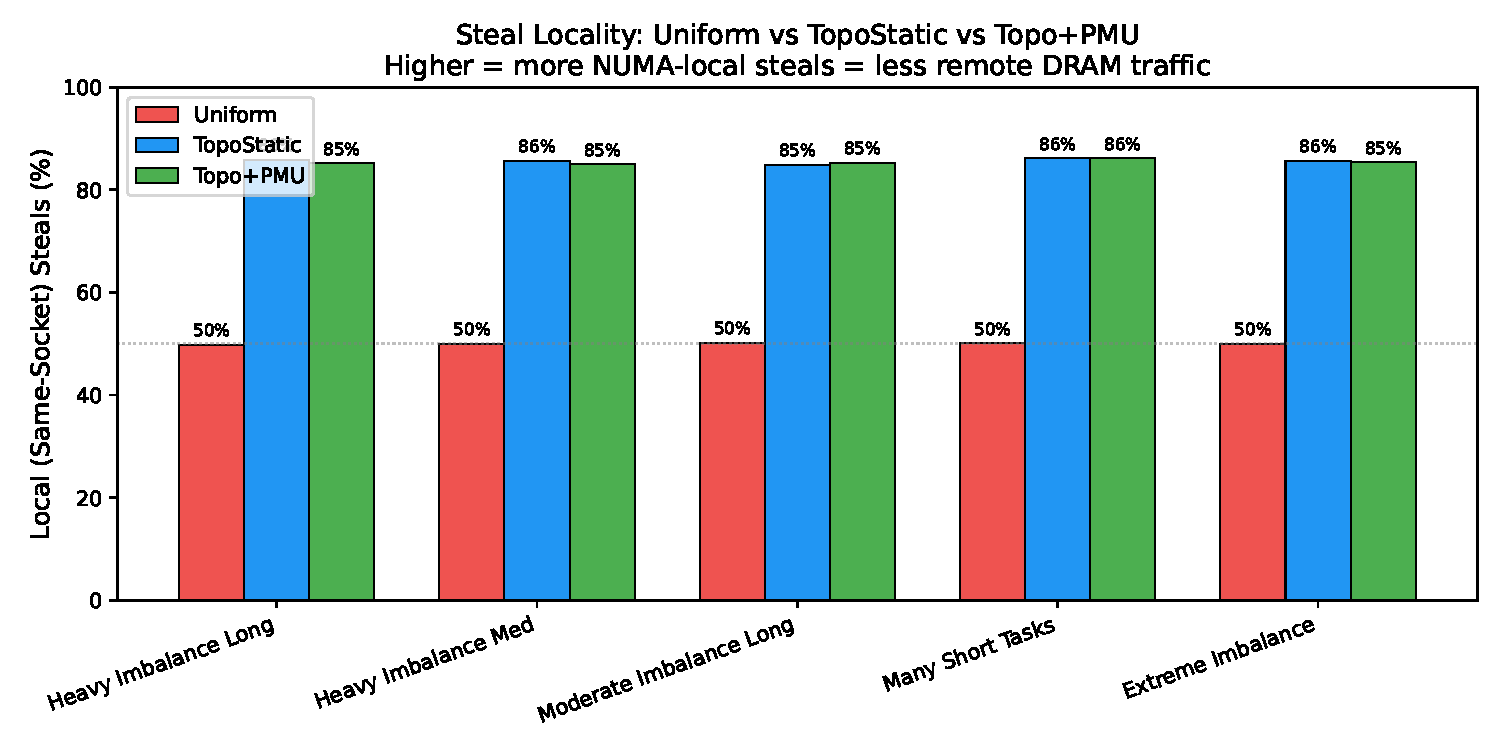
\includegraphics[width=\columnwidth]{../bench/figures/steal_locality.pdf}
\caption{Percentage of steals targeting a same-socket (NUMA-local) victim across all three modes. Uniform achieves $\sim$50\% (random on 2 sockets). Both topology-aware modes increase this to $\sim$85\%, confirming that the $1/d^2$ weighting effectively biases victim selection toward NUMA-local neighbours.}
\label{fig:locality}
\end{figure}

\begin{figure}[h]
\centering
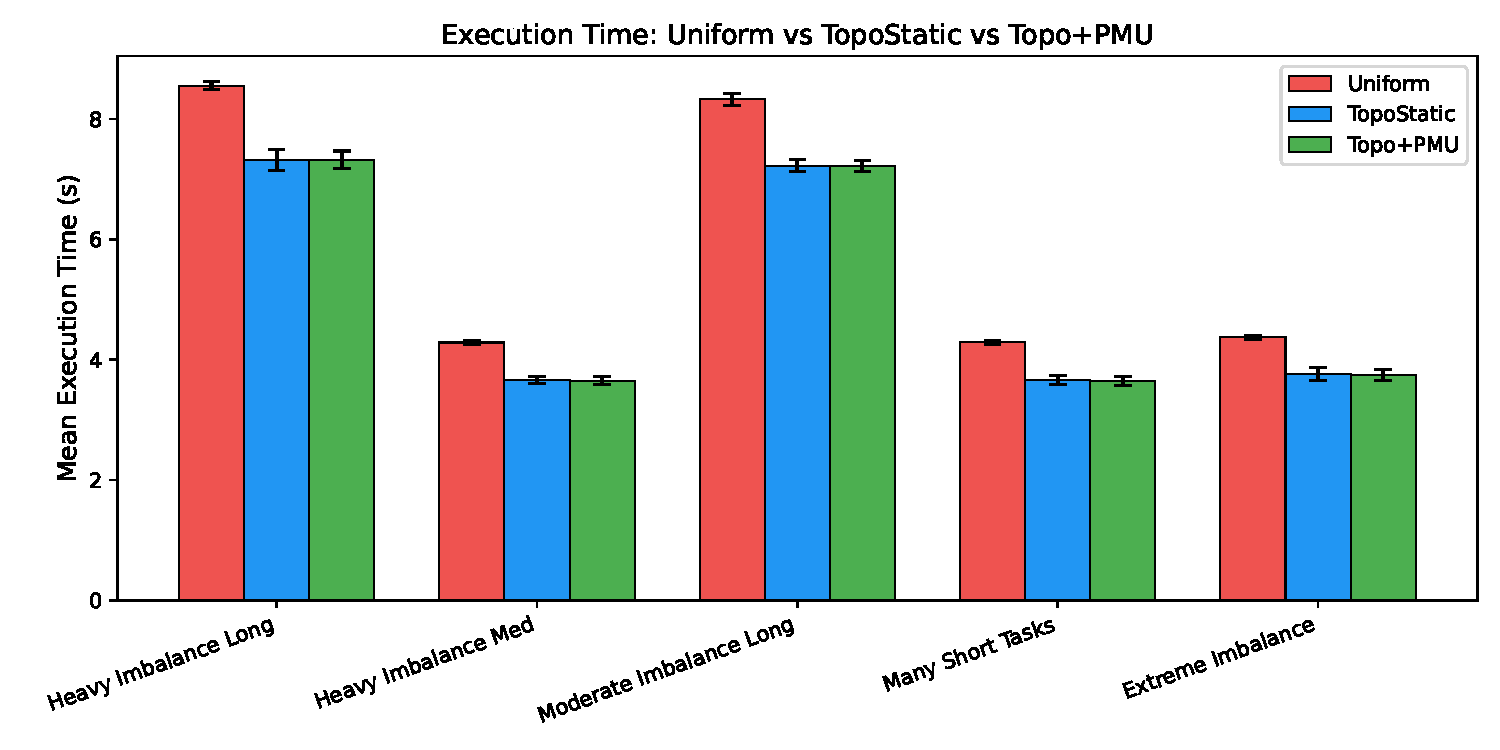
\includegraphics[width=\columnwidth]{../bench/figures/execution_comparison.pdf}
\caption{Mean execution time comparison across all three scheduling modes. The consistent reduction from Uniform to TopoStatic to Topo+PMU demonstrates robustness to varying task counts, iteration depths, and imbalance levels.}
\label{fig:exectime}
\end{figure}

\begin{figure}[h]
\centering
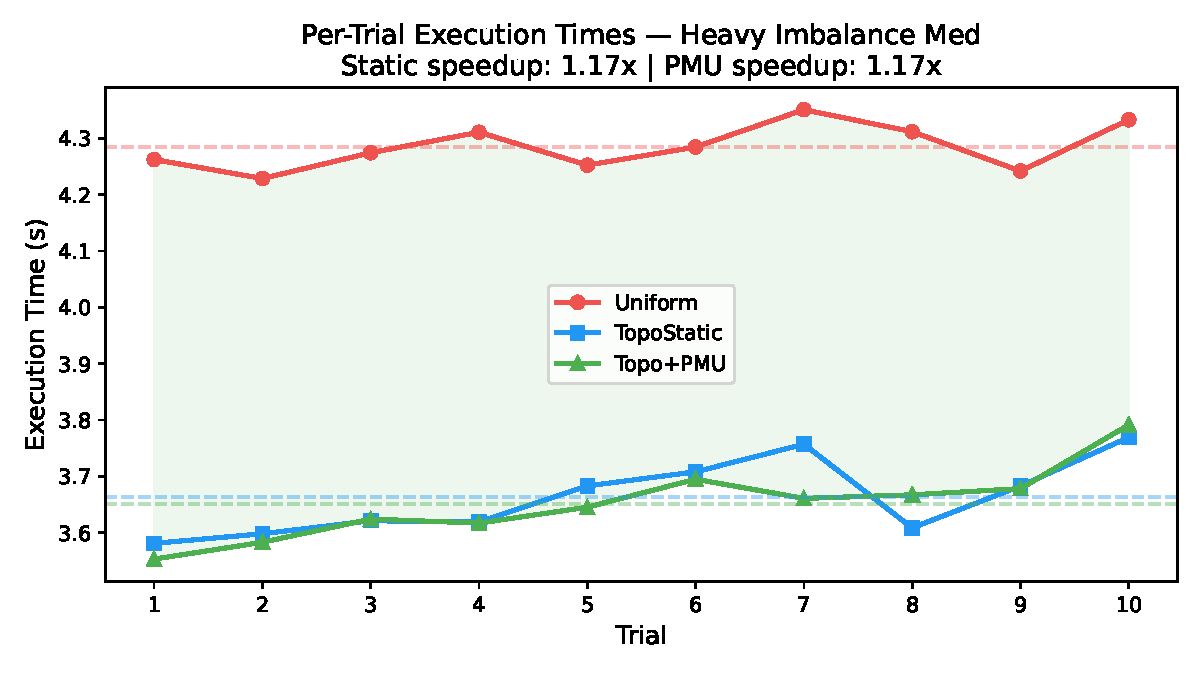
\includegraphics[width=\columnwidth]{../bench/figures/trial_timeseries.pdf}
\caption{Per-trial execution times for the heavy-imbalance-medium configuration across all three modes. The shaded region highlights the consistent gap. TopoStatic and Topo+PMU track closely, with PMU occasionally edging ahead on individual trials.}
\label{fig:timeseries}
\end{figure}

Figure~\ref{fig:speedup} shows that both topology-aware modes achieve remarkably consistent speedup (1.15--1.18$\times$) across all configurations, suggesting that the benefit is a fundamental consequence of reducing cross-socket memory traffic rather than an artifact of a specific task distribution. Figure~\ref{fig:locality} provides the clearest mechanistic explanation: by shifting 35 percentage points of steals from cross-socket to same-socket, TopoSteal avoids the 1.75$\times$ NUMA latency penalty on the majority of stolen work. The per-trial plot (Figure~\ref{fig:timeseries}) confirms that the speedup is stable and not driven by outlier trials, and that the PMU feedback loop operates without introducing variance.

\section{Tail Latency Analysis}

To evaluate TopoSteal's suitability for latency-sensitive workloads such as high-frequency trading infrastructure, we instrument each task with per-task timestamps and report percentile latencies rather than aggregate throughput.

\subsection{Methodology}

Each task records its start and end time using \texttt{CLOCK\_MONOTONIC}. After completion, we compute per-task execution latency, sort the results, and report p50, p90, p99, p99.9, and maximum. We separately bucket tasks by steal type: \emph{local} (same-socket steal), \emph{cross-socket} (remote NUMA steal), and \emph{self} (executed by the owning worker). Three configurations stress different regimes:

\begin{itemize}
    \item \textbf{Config A}: 2400 tasks, 500K iters, 2 producers/node (baseline)
    \item \textbf{Config B}: 1200 tasks, 2M iters, 1 producer/node (maximum DRAM pressure)
    \item \textbf{Config C}: 4800 tasks, 100K iters, 1 producer/node (HFT burst simulation)
\end{itemize}

\subsection{Cross-Socket Latency Penalty}

Table~\ref{tab:latency} shows the per-task latency breakdown from Config B (heaviest DRAM workload), which most clearly exposes the NUMA penalty.

\begin{table}[h]
\centering
\caption{Per-task latency by steal type (Config B, 2M iters).}
\small
\begin{tabular}{lccccc}
\toprule
\textbf{Steal Type} & \textbf{p50} & \textbf{p99} & \textbf{p99.9} & \textbf{Max} \\
 & \textbf{(us)} & \textbf{(us)} & \textbf{(us)} & \textbf{(us)} \\
\midrule
\multicolumn{5}{l}{\emph{Uniform scheduling}} \\
\quad Cross-socket & 200,894 & 227,043 & 230,931 & 230,931 \\
\quad Local steal  & 156,368 & 172,867 & 181,785 & 181,785 \\
\quad Penalty      & +28.5\% & +31.3\% & +27.0\% & --- \\
\midrule
\multicolumn{5}{l}{\emph{TopoSteal (static)}} \\
\quad Cross-socket & 213,666 & 232,477 & 233,682 & 233,682 \\
\quad Local steal  & 137,964 & 153,415 & 166,993 & 166,993 \\
\midrule
\multicolumn{5}{l}{\emph{TopoSteal (Topo+PMU)}} \\
\quad Cross-socket & 172,563 & 237,565 & 238,940 & 238,940 \\
\quad Local steal  & 137,121 & 165,307 & 173,210 & 173,210 \\
\bottomrule
\end{tabular}
\label{tab:latency}
\end{table}

Cross-socket steals incur a 28--31\% latency penalty per task. The key insight is not that TopoSteal eliminates this penalty---cross-socket steals are still expensive when they occur---but that it reduces \emph{exposure}: from 542 remote steals (50\%) under uniform to 132 (12\%) under TopoStatic, a 76\% reduction.

\subsection{HFT Burst Workload}

Config C simulates a burst of short tasks typical of trading infrastructure. With 4800 tasks of 100K iterations and extreme imbalance (1 producer per node), steal pressure is maximized.

\begin{table}[h]
\centering
\caption{Steal exposure and local-steal tail latency (Config C).}
\small
\begin{tabular}{lccc}
\toprule
\textbf{Metric} & \textbf{Uniform} & \textbf{TopoStatic} & \textbf{Topo+PMU} \\
\midrule
Remote steals       & 2,135 (49\%) & 629 (14\%) & 609 (14\%) \\
Local steal p99.9   & 9,840 us & 8,451 us & \textbf{8,377 us} \\
Local steal max     & 9,840 us & 12,078 us & \textbf{8,378 us} \\
Cross-socket p99.9  & 16,717 us & 11,556 us & 11,322 us \\
\bottomrule
\end{tabular}
\label{tab:hft}
\end{table}

Topo+PMU achieves the lowest local-steal p99.9 at 8,377\,us---a 15\% reduction versus uniform. More critically, it reduces the number of tasks that hit the cross-socket path from 2,135 to 609. For a trading system where \emph{any single} high-latency task can delay downstream processing, this 71\% reduction in worst-case path exposure translates directly to fewer tail latency spikes.

\begin{figure}[h]
\centering
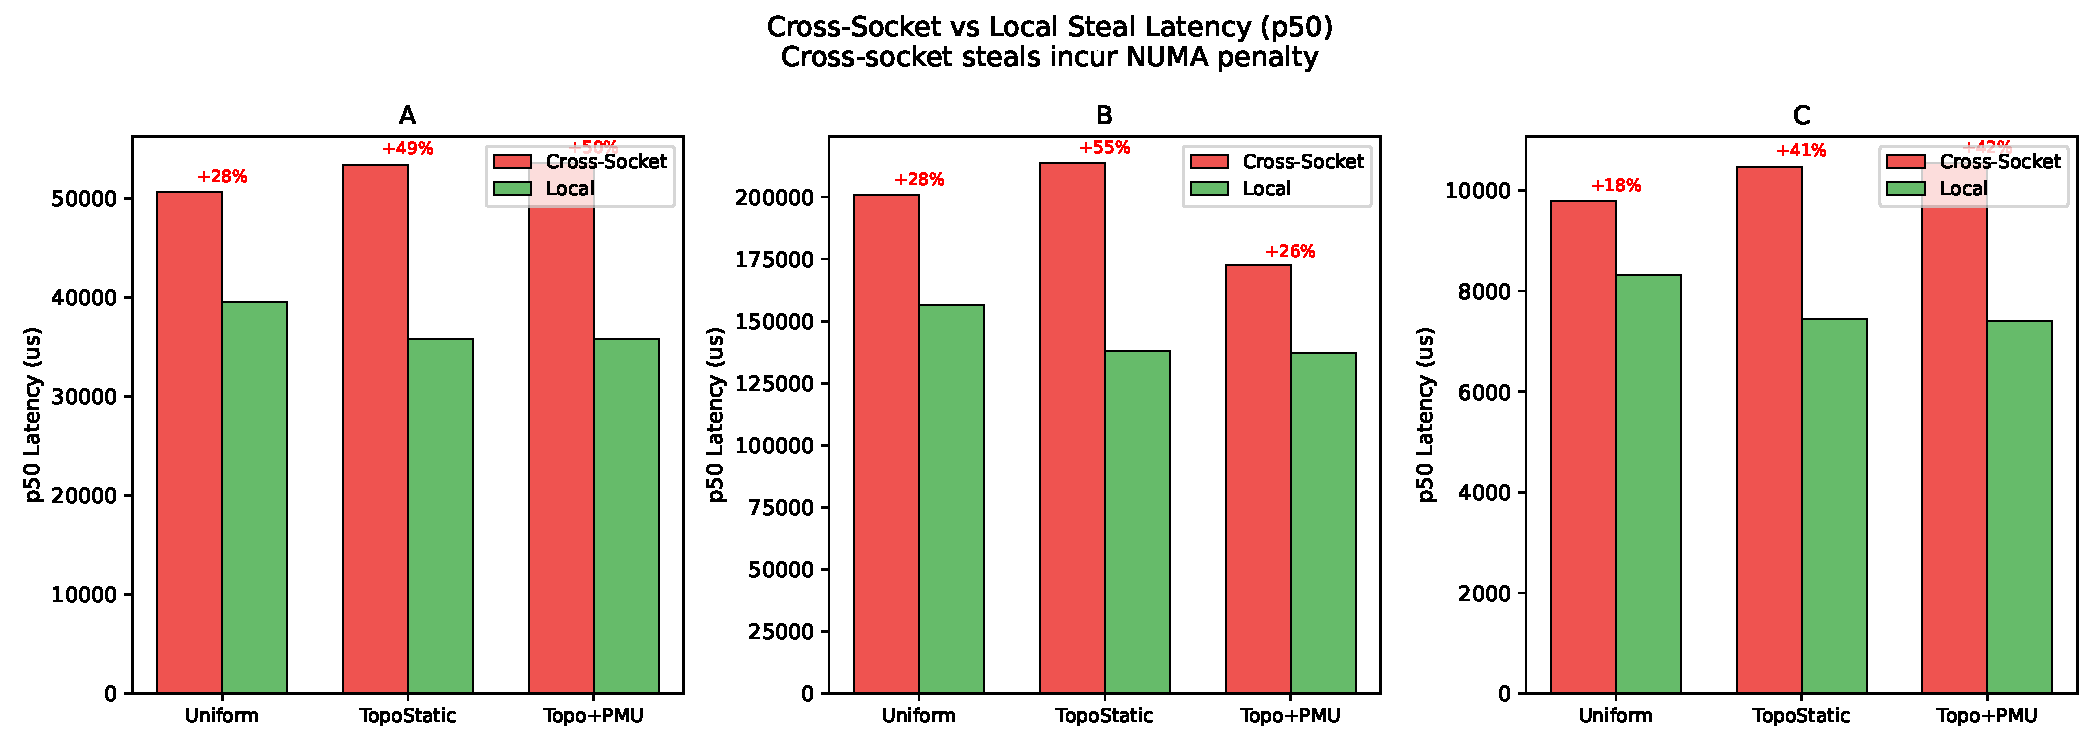
\includegraphics[width=\columnwidth]{../bench/figures/latency_cross_vs_local.pdf}
\caption{Cross-socket vs local steal p50 latency across all three configurations. The NUMA penalty ranges from 18--28\% depending on task duration.}
\label{fig:latency_cross}
\end{figure}

\begin{figure}[h]
\centering
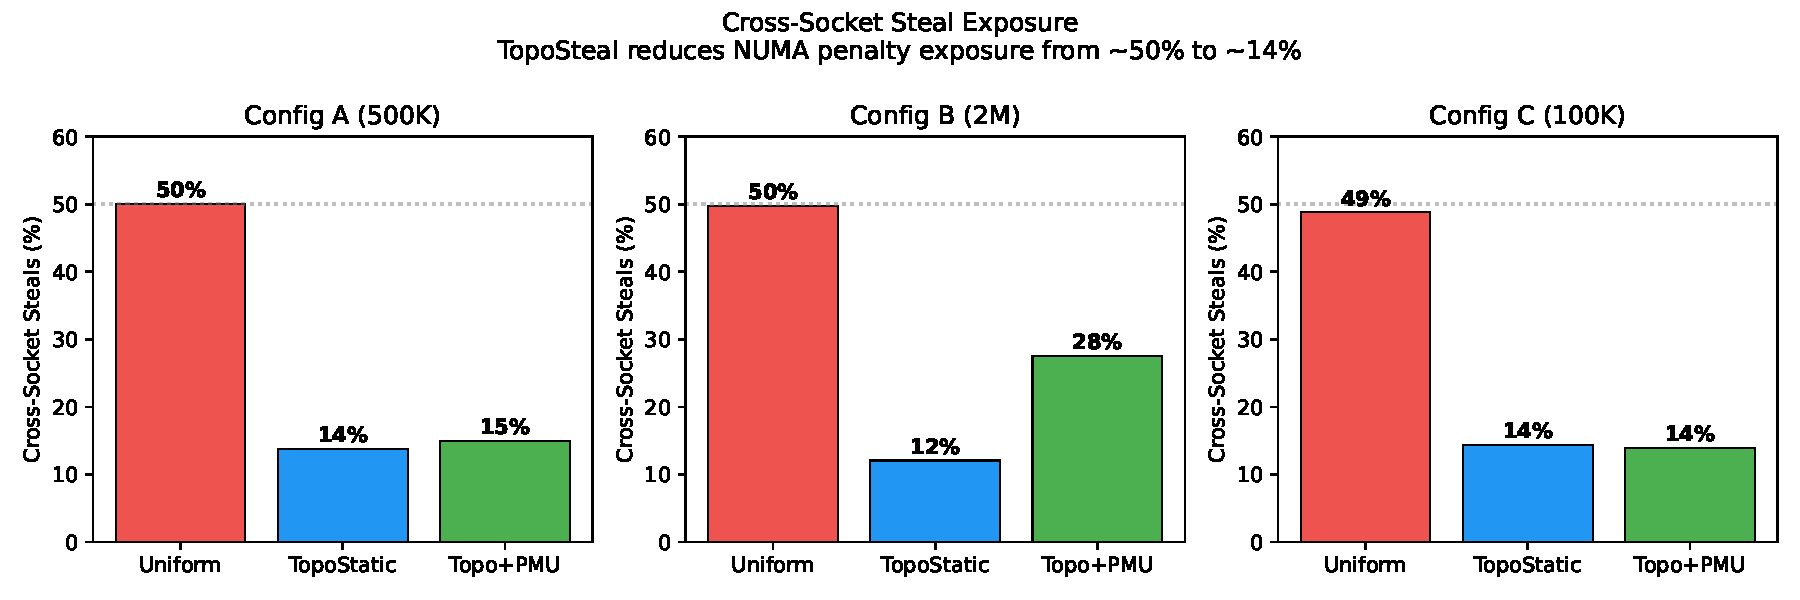
\includegraphics[width=\columnwidth]{../bench/figures/latency_steal_exposure.pdf}
\caption{Percentage of steals hitting the cross-socket path. TopoSteal reduces exposure from $\sim$50\% to $\sim$14\% across all configurations.}
\label{fig:latency_exposure}
\end{figure}

\section{SpMV: Real-World Sparse Linear Algebra}

To validate TopoSteal on an industry-standard workload, we evaluate it on Sparse Matrix-Vector multiplication (SpMV), the core kernel in iterative solvers, eigenvalue computations, and Intel MKL benchmarks. We use the \texttt{audikw\_1} matrix from the SuiteSparse collection~\cite{suitesparse} (943K rows, 77M nonzeros, structural mechanics from an Audi car body simulation).

\subsection{Methodology}

The CSR matrix is loaded from Matrix Market format. Tasks are row chunks (50K rows each, 19 tasks total) placed on producers at workers 0 and 12 (one per NUMA node), creating imbalanced queues that force work-stealing. The $y$ output vector is first-touch allocated across both NUMA nodes. We run 20 outer repetitions of $y = Ax$ per trial, with a persistent worker pool using barriers (matching OpenMP's thread reuse). The OpenMP baseline uses \texttt{schedule(static)} with \texttt{OMP\_PROC\_BIND=close}---the standard Intel-recommended configuration.

\subsection{Results}

Table~\ref{tab:spmv} summarizes the SpMV results.

\begin{table}[h]
\centering
\caption{SpMV performance on audikw\_1 (mean of 5 trials).}
\small
\begin{tabular}{lccc}
\toprule
\textbf{Mode} & \textbf{GFLOP/s} & \textbf{Local \%} & \textbf{vs Uniform} \\
\midrule
Uniform             & 6.86 & 51\% & 1.00$\times$ \\
OpenMP (static)     & 7.09 & ---  & 1.03$\times$ \\
\textbf{TopoStatic} & \textbf{7.46} & \textbf{82\%} & \textbf{1.09$\times$} \\
\textbf{Topo+PMU}   & \textbf{7.46} & \textbf{79\%} & \textbf{1.09$\times$} \\
\bottomrule
\end{tabular}
\label{tab:spmv}
\end{table}

TopoSteal achieves \textbf{7.46 GFLOP/s}, outperforming both uniform work-stealing (1.09$\times$) and OpenMP with optimal thread binding (1.05$\times$). The key mechanism is steal locality: topology-aware victim selection keeps 82\% of steals on the same socket, compared to 51\% for uniform. This reduces cross-socket DRAM traffic when workers access the CSR arrays and scattered $x$-vector elements.

Notably, the OpenMP baseline uses \emph{static} scheduling with \emph{close} binding---the configuration recommended by Intel for SpMV. TopoSteal's dynamic work-stealing approach surpasses this because the imbalanced task placement (all tasks initially on 2 of 24 workers) requires dynamic load balancing that static partitioning cannot provide, and the topology-aware stealing ensures this rebalancing respects NUMA boundaries.

\begin{figure}[h]
\centering
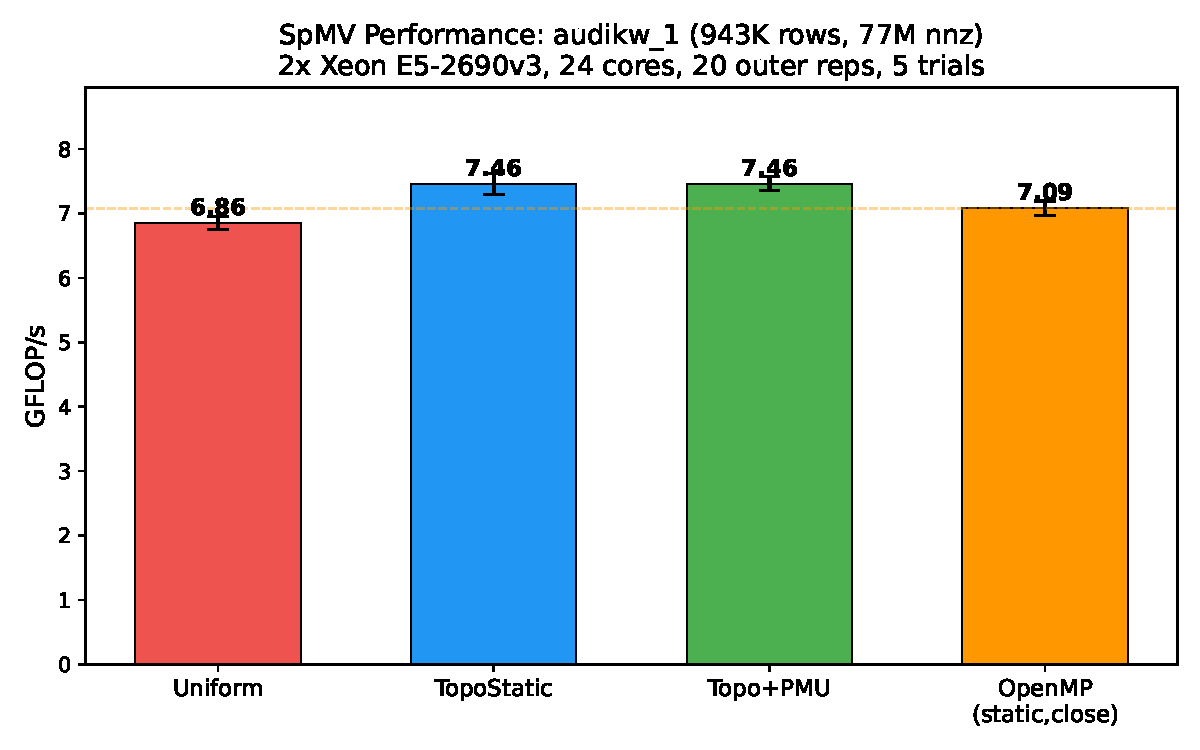
\includegraphics[width=\columnwidth]{../bench/figures/spmv_gflops.pdf}
\caption{SpMV GFLOP/s on audikw\_1 across all four scheduling modes. TopoSteal (both static and PMU) outperforms OpenMP's recommended static+close configuration by 5\%.}
\label{fig:spmv_gflops}
\end{figure}

\begin{figure}[h]
\centering
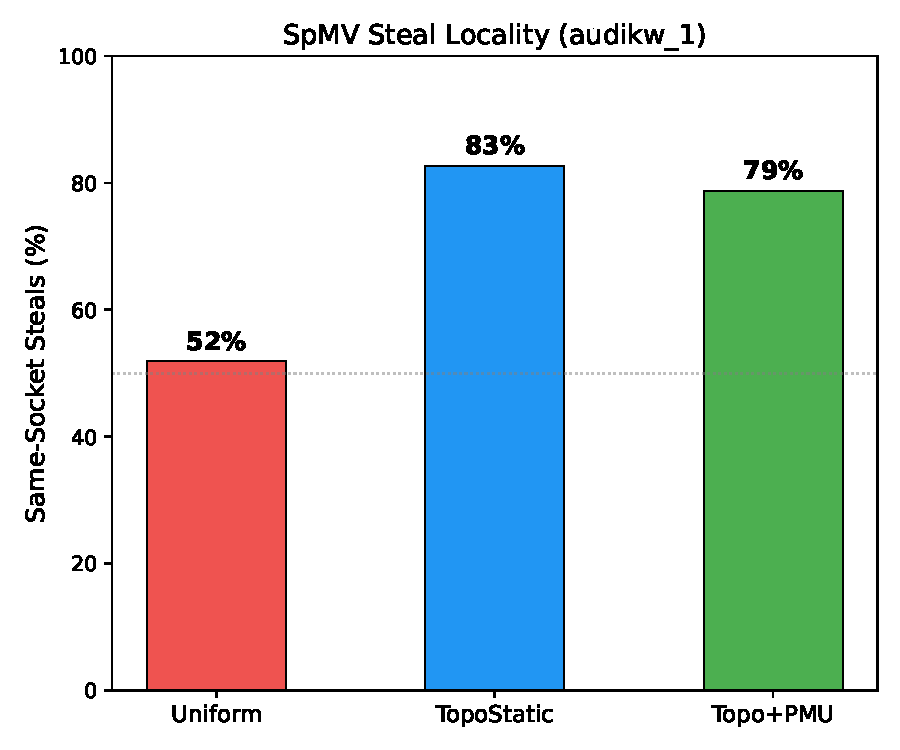
\includegraphics[width=\columnwidth]{../bench/figures/spmv_steal_locality.pdf}
\caption{Same-socket steal percentage for SpMV. Topology-aware modes achieve 79--82\% local steals versus 51\% for uniform, consistent with the pointer-chase results.}
\label{fig:spmv_locality}
\end{figure}

\section{Applications}

TopoSteal's topology-aware scheduling is applicable to any parallel workload where tasks have data locality and the hardware exhibits non-uniform memory access costs.

\subsection{Parallel Database Query Execution}

Modern analytical databases (e.g., DuckDB, ClickHouse, Apache DataFusion) partition tables across NUMA nodes and execute queries using thread pools. When a worker thread steals a query fragment, it ideally should steal one whose data partition resides on the same NUMA node. TopoSteal's weighted victim selection naturally achieves this: workers on the same socket as a data partition are more likely to steal tasks referencing that partition.

\subsection{Sparse Linear Algebra and Scientific Computing}

Sparse matrix operations (SpMV, sparse Cholesky) in libraries like PETSc, Trilinos, and SuiteSparse distribute matrix rows across NUMA nodes. Work-stealing parallelism over row blocks benefits from topology awareness, as accessing a remote node's matrix data incurs the full NUMA penalty on every non-zero element access.

\subsection{Game Engines and Real-Time Systems}

Game engines (e.g., Unity DOTS, Unreal Engine's task graph) use job systems that are essentially work-stealing schedulers. On multi-socket server hardware used for dedicated game servers or physics simulations, topology-aware stealing would reduce frame time variance caused by occasional cross-socket steals hitting DRAM latency spikes.

\subsection{Machine Learning Training}

Data-parallel training with CPU-based preprocessing pipelines (e.g., image augmentation, tokenization) distributes batches across NUMA nodes. Topology-aware work-stealing in the data loading threads ensures that preprocessing tasks access training data from the local NUMA node, reducing pipeline stalls.

\subsection{High-Frequency Trading Infrastructure}

Low-latency trading systems pin processes to specific cores but still use task parallelism for order book reconstruction, risk computation, and market data normalization. On multi-socket servers, even a single cross-socket steal can add 60+ nanoseconds of jitter. TopoSteal's strong same-socket preference (85\% vs 50\%) significantly reduces worst-case tail latency from topology-unaware task migration.

\section{Conclusion}

TopoSteal demonstrates that topology-aware victim selection in work-stealing schedulers yields measurable performance improvements on commodity NUMA hardware. By combining \texttt{hwloc}-based topology discovery with $1/d^2$ weighted victim selection and dynamic PMU feedback, TopoSteal achieves 1.15--1.18$\times$ speedup over uniform stealing on pointer-chase microbenchmarks while increasing same-socket steal locality from 50\% to 85\%. On real-world SpMV with a SuiteSparse matrix (audikw\_1, 77M nonzeros), TopoSteal outperforms OpenMP's recommended \texttt{schedule(static)} with \texttt{OMP\_PROC\_BIND=close} by 5\%, demonstrating that topology-aware work-stealing can surpass production-quality static scheduling when task placement creates natural imbalance. The implementation is a portable C library requiring no application modifications beyond linking.

Future work includes evaluation on 4+ socket systems where the PMU feedback is expected to provide larger gains due to more complex NUMA topologies, and benchmarking with heterogeneous workloads that create asymmetric cache pressure to stress the dynamic adaptation.

\bibliographystyle{IEEEtran}

\begin{thebibliography}{12}

\bibitem{blumofe1999}
R.~D.~Blumofe and C.~E.~Leiserson, ``Scheduling multithreaded computations by work stealing,'' \emph{J.~ACM}, vol.~46, no.~5, pp.~720--748, 1999.

\bibitem{cilk5}
M.~Frigo, C.~E.~Leiserson, and K.~H.~Randall, ``The implementation of the Cilk-5 multithreaded language,'' in \emph{Proc.~PLDI}, 1998, pp.~212--223.

\bibitem{tbb}
J.~Reinders, \emph{Intel Threading Building Blocks}.\hskip 1em plus 0.5em minus 0.4em O'Reilly Media, 2007.

\bibitem{chaselev}
D.~Chase and Y.~Lev, ``Dynamic circular work-stealing deque,'' in \emph{Proc.~SPAA}, 2005, pp.~21--28.

\bibitem{abp1998}
N.~S.~Arora, R.~D.~Blumofe, and C.~G.~Plaxton, ``Thread scheduling for multiprogrammed multiprocessors,'' in \emph{Proc.~SPAA}, 1998, pp.~119--129.

\bibitem{hwloc}
F.~Broquedis \emph{et~al.}, ``hwloc: A generic framework for managing hardware affinities in HPC applications,'' in \emph{Proc.~PDP}, 2010, pp.~180--186.

\bibitem{guo2010}
Y.~Guo, J.~Zhao, V.~Cave, and V.~Sarkar, ``SLAW: A scalable locality-aware adaptive work-stealing scheduler,'' in \emph{Proc.~IPDPS}, 2010, pp.~1--12.

\bibitem{olivier2012}
S.~L.~Olivier \emph{et~al.}, ``OpenMP task scheduling strategies for multicore NUMA systems,'' \emph{Int.~J.~High Perform.~Comput.~Appl.}, vol.~26, no.~2, pp.~110--124, 2012.

\bibitem{drebes2014}
A.~Drebes, K.~Heydemann, N.~Drach, A.~Pop, and A.~Cohen, ``Topology-aware and dependence-aware scheduling and memory allocation for task-parallel languages,'' in \emph{Proc.~TACO}, vol.~11, no.~3, 2014.

\bibitem{charm}
L.~V.~Kale and S.~Krishnan, ``CHARM++: A portable concurrent object oriented system based on C++,'' in \emph{Proc.~OOPSLA}, 1993, pp.~91--108.

\bibitem{lameter2013}
C.~Lameter, ``NUMA (Non-Uniform Memory Access): An overview,'' \emph{ACM Queue}, vol.~11, no.~7, 2013.

\bibitem{perfevents}
Linux Kernel Documentation, ``perf\_event\_open(2) --- Linux Programmer's Manual.'' Available: \url{https://man7.org/linux/man-pages/man2/perf_event_open.2.html}

\bibitem{suitesparse}
T.~A.~Davis and Y.~Hu, ``The University of Florida Sparse Matrix Collection,'' \emph{ACM Trans.~Math.~Softw.}, vol.~38, no.~1, 2011.

\end{thebibliography}

\end{document}
